\section{Overview}
Our system implements a classic three-tier architecture with clear separation of concerns:

\begin{enumerate}
    \item \textbf{Presentation Layer (Front-end)}: User interface for visualization and interaction
    \item \textbf{Logic Layer (Back-end)}: Business logic processing and data manipulation
    \item \textbf{Data Layer (Database)}: Storage and retrieval of blockchain transaction data
\end{enumerate}

The system follows a microservice architecture pattern with a poly-repo development approach. The codebase is split into separate repositories:
\begin{itemize}
    \item \textbf{\href{https://github.com/SwinHCMC-COS30049/cos30049-fe}{cos30049-fe}}: Frontend repository containing the NextJS application
    \item \textbf{\href{https://github.com/SwinHCMC-COS30049/cos30049-be}{cos30049-be}}: Backend repository containing the NestJS application
\end{itemize}
\section{Project Structure}
\begin{tcolorbox}[width=\textwidth, boxrule=0pt, colback=gray!5, colframe=gray!5, arc=0mm, outer arc=0mm]
\begin{lstlisting}[numbers=none]
/
|-- src/
|   |-- main.ts                # Application entry point
|   |-- common/                # Shared utilities and middleware
|   |   |-- decorators/        # Custom decorators
|   |   |-- filters/           # Exception filters
|   |   |-- guards/            # Authorization guards
|   |   |-- interceptors/      # Response transformers
|   |   |-- logger/            # Logging configuration
|   |   |-- seeder/            # Database seeders
|   |-- modules/               # Feature modules
|   |   |-- app.module.ts      # Root module
|   |   |-- auth/              # Authentication
|   |   |-- user/              # User management
|   |   |-- wallet/            # Wallet operations
|   |   |-- transaction/       # Transaction handling
|   |   |-- currency/          # Currency information
|   |   |-- exchange-rate/     # Exchange rate data
|   |   |-- edgedb/            # EdgeDB connection
|   |   |-- neo4j/             # Neo4j connection
|   |-- scripts/               # Utility scripts
|-- dbschema/                  # EdgeDB schema definitions
|   |-- default.esdl           # Main schema file
|   |-- migrations/            # Database migrations
|   |-- edgeql-js/             # Generated EdgeDB queries
|-- dist/                      # Compiled output
|-- node_modules/              # Dependencies
|-- docs/                      # Documentation
|-- .env                       # Environment variables
|-- package.json               # Project metadata and scripts
|-- tsconfig.json              # TypeScript configuration
|-- README.md                  # Project overview
\end{lstlisting}
\end{tcolorbox}
\section{API Architecture Diagram}
\begin{figure}[h]
    \centering
    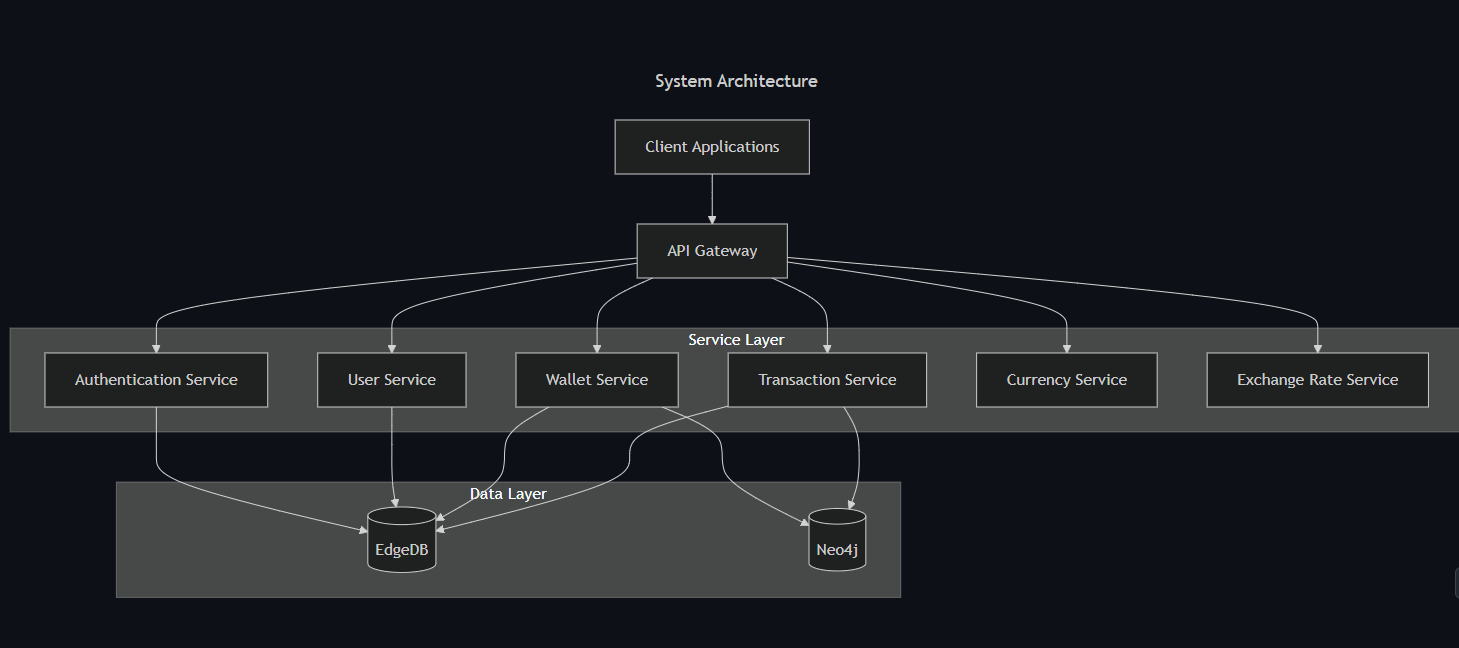
\includegraphics[width=\textwidth, keepaspectratio]{figures/architecture diagram.png}
    \caption{Architecture Diagram}
    \label{fig:Architecture Diagram}
\end{figure}
The architecture (Figure \ref{fig:Architecture Diagram} follows a multi-layered design pattern with clear separation of concerns. It consists of four main layers:

\subsection{Client Layer}
\begin{itemize}
  \item The top layer shows ``Client Applications'' which represent the user-facing interfaces that interact with the system
  \item These applications send requests to the backend services through the API Gateway
\end{itemize}

\subsection{API Gateway Layer}
\begin{itemize}
  \item Serves as the single entry point for all client requests
  \item Handles routing, request aggregation, and potentially authentication/authorization
  \item Directs traffic to the appropriate microservices in the Service Layer below
\end{itemize}

\subsection{Service Layer}
Contains six distinct microservices:
\begin{itemize}
  \item \textbf{Authentication Service}: Manages user identity, login, and security tokens
  \item \textbf{User Service}: Handles user profile management and preferences
  \item \textbf{Wallet Service}: Manages blockchain wallets and associated keys
  \item \textbf{Transaction Service}: Processes blockchain transactions and their metadata
  \item \textbf{Currency Service}: Handles different cryptocurrencies and their specifications
  \item \textbf{Exchange Rate Service}: Provides current and historical exchange rate data
\end{itemize}

\subsection{Data Layer}
Contains two different database systems:
\begin{itemize}
  \item \textbf{EdgeDB}: A graph-relational database that appears to store user, authentication, and possibly wallet data
  \item \textbf{Neo4j}: A graph database that likely stores transaction data, enabling complex relationship queries between transactions
\end{itemize}

\section{Data Flow}
The connections between layers show the flow of data:
\begin{itemize}
  \item Authentication and User services connect to EdgeDB
  \item Wallet and Transaction services connect to both EdgeDB and Neo4j
  \item This dual-database approach suggests different data access patterns for different types of information
\end{itemize}
% system_architecture.tex

\section{Authentication Flow}
\begin{figure}[h]
    \centering
    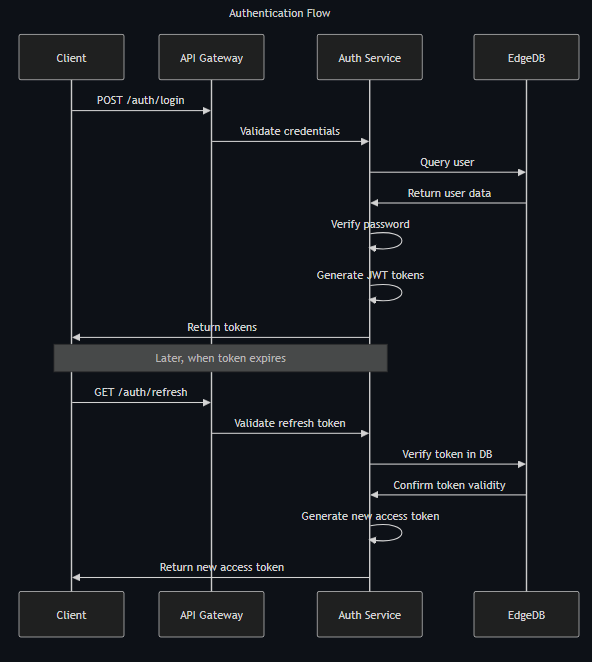
\includegraphics[width=\textwidth, keepaspectratio]{figures/authentication_flow.png}
    \caption{Authentication Flow}
    \label{fig:Authentication Flow}
\end{figure}

The authentication flow diagram (Figure \ref{fig:Authentication Flow}) illustrates a secure, token-based authentication system consisting of four key components: Client, API Gateway, Auth Service, and EdgeDB. The flow is divided into two main processes: initial authentication and token refresh.

\subsection{Initial Authentication Process}

\begin{enumerate}
    \item \textbf{Client Request Initiation}:
    \begin{itemize}
        \item The process begins when the Client sends a POST request to the ``/auth/login'' endpoint of the API Gateway.
        \item This request contains the user's credentials (likely username/email and password).
    \end{itemize}
    
    \item \textbf{Credential Validation}:
    \begin{itemize}
        \item The API Gateway forwards these credentials to the Auth Service for validation.
        \item The Auth Service serves as the central authentication authority in this architecture.
    \end{itemize}
    
    \item \textbf{User Data Retrieval}:
    \begin{itemize}
        \item To validate credentials, the Auth Service queries the EdgeDB database.
        \item EdgeDB returns the user's data, which likely includes the stored password hash and possibly user roles or permissions.
    \end{itemize}
    
    \item \textbf{Password Verification}:
    \begin{itemize}
        \item The Auth Service verifies the provided password against the stored password information.
        \item This likely uses secure hashing techniques to compare passwords without storing them in plaintext.
    \end{itemize}
    
    \item \textbf{JWT Token Generation}:
    \begin{itemize}
        \item Upon successful verification, the Auth Service generates JWT (JSON Web Tokens).
        \item These tokens typically include:
        \begin{itemize}
            \item An access token (short-lived) for API resource access
            \item A refresh token (longer-lived) for obtaining new access tokens
        \end{itemize}
    \end{itemize}
    
    \item \textbf{Token Response}:
    \begin{itemize}
        \item The Auth Service returns these tokens to the Client via the API Gateway.
        \item The Client stores these tokens for subsequent requests to the blockchain visualization system.
    \end{itemize}
\end{enumerate}

\subsection{Token Refresh Process}

\begin{enumerate}
    \item \textbf{Refresh Request}:
    \begin{itemize}
        \item When the access token expires, the Client sends a GET request to ``/auth/refresh''.
        \item This request includes the previously issued refresh token.
    \end{itemize}
    
    \item \textbf{Refresh Token Validation}:
    \begin{itemize}
        \item The API Gateway forwards the refresh token to the Auth Service.
        \item The Auth Service validates the refresh token's integrity and expiration.
    \end{itemize}
    
    \item \textbf{Database Verification}:
    \begin{itemize}
        \item The Auth Service verifies the token against records in EdgeDB.
        \item This step ensures the token hasn't been revoked or invalidated.
    \end{itemize}
    
    \item \textbf{Token Validity Confirmation}:
    \begin{itemize}
        \item EdgeDB confirms the token's validity status back to the Auth Service.
    \end{itemize}
    
    \item \textbf{New Access Token Generation}:
    \begin{itemize}
        \item Upon confirmation, the Auth Service generates a new access token.
        \item This process allows continuous authentication without requiring users to re-enter credentials.
    \end{itemize}
    
    \item \textbf{Token Return}:
    \begin{itemize}
        \item The new access token is returned to the Client via the API Gateway.
        \item The Client can now continue accessing the blockchain transaction visualization system.
    \end{itemize}
\end{enumerate}
This authentication architecture provides a robust security layer for the blockchain transaction information visualization system, ensuring that only authenticated users can access sensitive blockchain data while maintaining a seamless user experience.
\section{Transaction Query Process}
\begin{figure}[h]
    \centering
    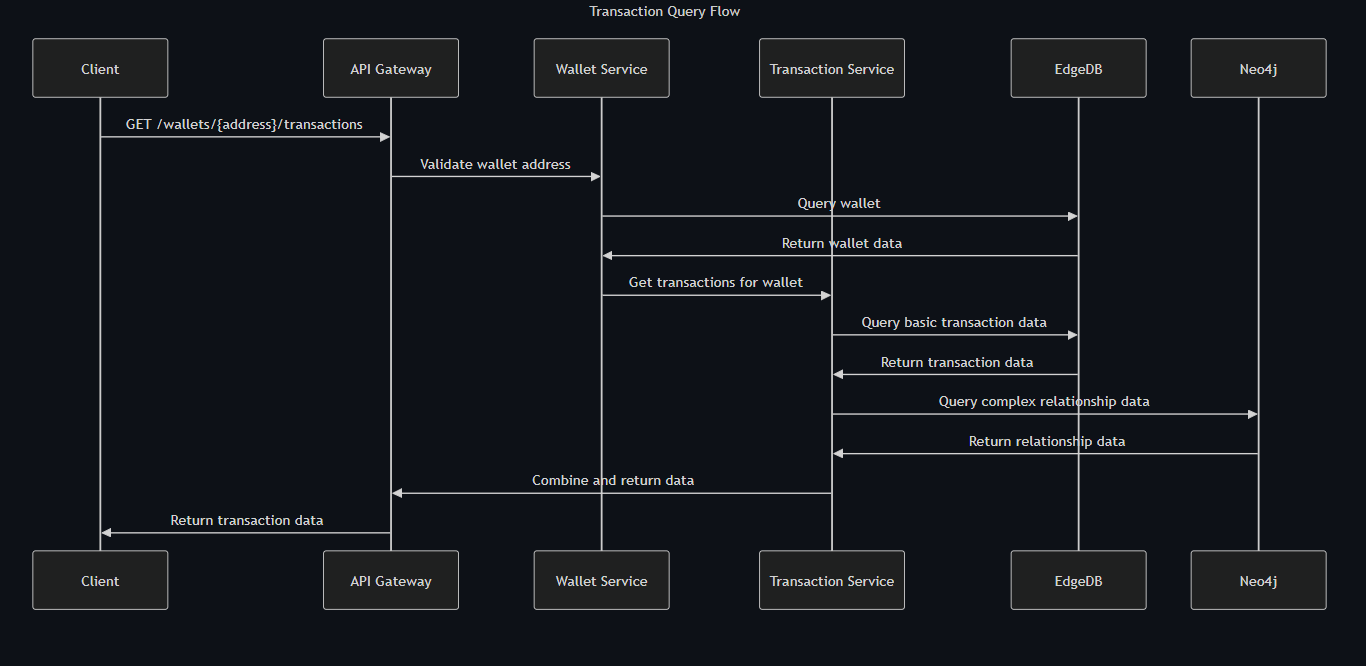
\includegraphics[width=\textwidth, keepaspectratio]{figures/_query.png}
    \caption{Transaction Query}
    \label{fig:Transaction Query}
\end{figure}
This diagram ,see Figure \ref{fig:Transaction Query}, illustrates the comprehensive transaction query process of the blockchain visualization system, showing how transaction data is retrieved and processed through a microservices architecture. The flow involves six key components: Client, API Gateway, Wallet Service, Transaction Service, EdgeDB, and Neo4j:

\begin{enumerate}
    \item \textbf{Client Request Initiation}:
    \begin{itemize}
        \item The flow begins when the Client sends a GET request to ``/wallets/\{address\}/transactions'' through the API Gateway.
        \item This endpoint is designed to retrieve all transactions associated with a specific blockchain wallet address.
    \end{itemize}
    
    \item \textbf{Wallet Address Validation}:
    \begin{itemize}
        \item The API Gateway forwards the request to the Wallet Service.
        \item The Wallet Service performs validation on the provided wallet address to ensure it's correctly formatted and potentially exists in the system.
    \end{itemize}
    
    \item \textbf{Wallet Data Retrieval}:
    \begin{itemize}
        \item The Transaction Service queries EdgeDB to retrieve wallet information.
        \item EdgeDB returns the wallet data, which likely includes wallet metadata, balance information, and wallet status.
    \end{itemize}
    
    \item \textbf{Transaction Retrieval}:
    \begin{itemize}
        \item After confirming the wallet exists, the Transaction Service requests transactions associated with this wallet.
        \item This step involves querying basic transaction data from EdgeDB, which likely stores the fundamental transaction records.
    \end{itemize}
    
    \item \textbf{Basic Transaction Data Return}:
    \begin{itemize}
        \item EdgeDB returns the basic transaction data to the Transaction Service.
        \item This data typically includes transaction hashes, timestamps, values, and basic sender/receiver information.
    \end{itemize}
    
    \item \textbf{Complex Relationship Query}:
    \begin{itemize}
        \item The Transaction Service then queries Neo4j database for complex relationship data.
        \item Neo4j, being a graph database, is particularly suited for handling complex relationships between blockchain entities.
        \item This step retrieves additional contextual information about the transactions, such as:
        \begin{itemize}
            \item Transaction patterns
            \item Connected wallets in the transaction network
            \item Historical relationships between addresses
            \item Potentially suspicious activity patterns
        \end{itemize}
    \end{itemize}
    
    \item \textbf{Relationship Data Return}:
    \begin{itemize}
        \item Neo4j returns the relationship data to the Transaction Service.
        \item This data enriches the basic transaction information with network context.
    \end{itemize}
    
    \item \textbf{Data Aggregation and Processing}:
    \begin{itemize}
        \item The Transaction Service combines the basic transaction data from EdgeDB with the complex relationship data from Neo4j.
        \item This combined dataset provides a comprehensive view of the wallet's transaction history within its network context.
    \end{itemize}
    
    \item \textbf{Final Response}:
    \begin{itemize}
        \item The processed and aggregated data is sent back through the Wallet Service to the API Gateway.
        \item Finally, the API Gateway returns the complete transaction data to the Client.
    \end{itemize}
\end{enumerate}

\section{Key Design Decisions}
\subsection{Dual Database Approach}
\textbf{Decision:} Use both EdgeDB and Neo4j for different aspects of data storage and querying.

\textbf{Rationale:}
\begin{itemize}
\item EdgeDB provides strong typing and schema validation for structured data
\item Neo4j excels at relationship queries needed for transaction graph analysis
\item This combination offers the best of both worlds for cryptocurrency data
\end{itemize}
\subsection{Modular Architecture}
\textbf{Decision:} Organize code into feature modules following NestJS best practices.

\textbf{Rationale:}
\begin{itemize}
\item Improves maintainability by separating concerns
\item Enables independent development of features
\item Facilitates testing and code reuse
\end{itemize}
\subsection{JWT Authentication}
\textbf{Decision:} Use JWT tokens with refresh token rotation for authentication.

\textbf{Rationale:}
\begin{itemize}
\item Stateless authentication reduces database load
\item Refresh tokens enable longer sessions without compromising security
\item Industry standard approach for API authentication
\end{itemize}
\subsection{API Documentation with Swagger}
\textbf{Decision:} Automatically generate API documentation using Swagger.

\textbf{Rationale:}
\begin{itemize}
\item Keeps documentation in sync with code
\item Provides interactive testing interface
\item Improves developer experience
\end{itemize}
\section{Performance Considerations}
\begin{enumerate}
\item \textbf{Database Indexing}: Critical fields like wallet addresses and transaction hashes are indexed for fast lookups.
\item \textbf{Caching Strategy}: Frequently accessed data like exchange rates can be cached to reduce database load.
\item \textbf{Pagination}: All list endpoints support pagination to handle large datasets efficiently.
\item \textbf{Query Optimization}: Complex graph queries are optimized to minimize processing time.
\end{enumerate}
\section{Security Measures}
\begin{enumerate}
    \item \textbf{Authentication}: JWT-based authentication with proper token expiration.
    \item \textbf{Password Handling}: Passwords are hashed using bcrypt before storage.
    \item \textbf{Input Validation}: All inputs are validated using Zod schemas.
    \item \textbf{Rate Limiting}: API endpoints are protected against abuse with rate limiting.
    \item \textbf{CORS Configuration}: Cross-Origin Resource Sharing is properly configured.
\end{enumerate}
\section{Deployment Strategy}
The application is designed to be deployed in a containerized environment using Docker, with separate containers for:
\begin{enumerate}
    \item NestJS API
    \item EdgeDB database
    \item Neo4j database
\end{enumerate}
This enables easy scaling of individual components as needed.